\documentclass{article}
\usepackage{graphicx} % Required for inserting images
\usepackage{float}
\usepackage[T1]{fontenc}
\usepackage{amsmath}
\usepackage[margin=1in]{geometry}
\usepackage{booktabs}
\usepackage{tabularx}
\usepackage[hidelinks]{hyperref}

\title{Tilting the stress-sized put book toward high-VVIX days}
\author{Experiment report \textperiodcentered{} L/S Gamma Desk, QUANTT}
\date{2026-11-02}

\begin{document}

\maketitle

\textbf{Question:} On the 35\% stress-sized \texttt{hedged} book, does scaling each entry's stress budget by VVIX's one-year percentile (0.5x on the calmest VVIX days, 1.5x on the most volatile) earn more net P\&L than the fixed 35\% budget, at 1x and 2x spreads, over the full window and in each half, without a worse tail or a drawdown beyond \$87,500?

\textbf{Method:}

\begin{itemize}

\item \textbf{Pre-registration:} the hypothesis card was committed before any run (commit 457e2b6). The research switches \texttt{size\_\allowbreak{}by} and \texttt{size\_\allowbreak{}tilt} were committed before it, in 73e16a4.

\item \textbf{Data:} the live paper rules (\texttt{configs/\allowbreak{}paper.\allowbreak{}toml}) are replayed on R2 replay snapshots v1 (config\_hash b040760187f0) over the development window 2014-06-02 to 2024-12-31. The hold-out (2025-01-01 to 2026-07-10) was not used.

\item \textbf{Book:} every variant is the \texttt{hedged} book of 2026-10-22-stress-sized-puts.

\begin{itemize}

\item An always-on short 25-delta put, with the signal ignored and the flat exit off.

\item Sized at each entry to the most contracts whose loss in a one-day 20\% SPY drop, with IV at max(60\%, the put's IV), stays within the budget.

\item Hedged daily with a 10-share band. Stop at 1x the credit, profit-take at 50\% and time exit at 7 DTE.

\end{itemize}

\item \textbf{Tilt:} the budget is 35\% \ensuremath{\times} (1 + tilt \ensuremath{\times} (2p \ensuremath{-} 1)), where p is the percentile of the prior day's VVIX close among its last 252 closes.

\item \textbf{Variants:}

\begin{itemize}

\item \texttt{vvix} (primary): tilt 0.5, a budget of 17.5\% to 52.5\% of capital;

\item \texttt{vvix\_\allowbreak{}light}: tilt 0.25;

\item \texttt{vvix\_\allowbreak{}reverse}: tilt \ensuremath{-}0.5, larger when VVIX is low.

\end{itemize}

\item \textbf{Comparison:} the registered \texttt{2026-\allowbreak{}10-\allowbreak{}22-\allowbreak{}stress-\allowbreak{}sized-\allowbreak{}puts/\allowbreak{}hedged} runs at the same spread multiple, reused and not rerun. With the new switches off, the engine reproduces that book's equity exactly.

\item \textbf{Costs and schedule:} every variant was run at 1x and 2x spreads. \$0.65 per contract and \$0.005 per share, with a \$1 minimum per order. Decisions, exits and hedges run once a day at 10:15 ET.

\end{itemize}

This report was written by Claude at the PM's request.

\section{Result vs the pass bar}

Every check had to hold at 1x and 2x. P\&L is net of costs in USD. ES is the mean of the worst 5\% of daily P\&L.

\begin{center}\small
\begin{tabularx}{\linewidth}{>{\raggedright\arraybackslash}X l l l l >{\raggedright\arraybackslash}X}
\toprule
\textbf{Check (\texttt{vvix} vs \texttt{hedged})} & \textbf{1x value} & \textbf{1x bar} & \textbf{2x value} & \textbf{2x bar} & \textbf{Result} \\
\midrule
Net P\&L, full window & \$145,183 & > \$121,482 & \$130,641 & > \$101,172 & pass \\
Net P\&L, 2014-06 to 2019-12 & \$46,997 & > \$49,132 & \$46,658 & > \$42,687 & \textbf{fail (1x)} \\
Net P\&L, 2020-01 to 2024-12 & \$98,186 & > \$72,350 & \$83,984 & > \$58,485 & pass \\
ES 5\% within 1.10x & \ensuremath{-}\$3,589 & \ensuremath{\geq} \ensuremath{-}\$3,317 & \ensuremath{-}\$3,619 & \ensuremath{\geq} \ensuremath{-}\$3,404 & \textbf{fail} \\
Max drawdown \ensuremath{\leq} \$87,500 & \$106,599 & \ensuremath{\leq} \$87,500 & \$110,464 & \ensuremath{\leq} \$87,500 & \textbf{fail} \\
Round trips (floor \ensuremath{\geq} 30) & 181 &  &  &  & met \\
\bottomrule
\end{tabularx}
\end{center}

\textbf{Verdict: failed.} The VVIX tilt earned more (\$23.7k at 1x, \$29.5k at 2x), but it bought that with a bigger crash.

\begin{itemize}

\item Its drawdown broke the \$87,500 stress budget at both spreads.

\item Its tail was 1.19x /\allowbreak{} 1.17x the fixed budget's at 1x /\allowbreak{} 2x.

\item It lost to the fixed budget in 2014-2019 at 1x.

\end{itemize}

\subsection{Full-window numbers (not part of the bar)}

\begin{center}\small
\begin{tabularx}{\linewidth}{>{\raggedright\arraybackslash}X >{\raggedright\arraybackslash}X >{\raggedright\arraybackslash}X >{\raggedright\arraybackslash}X >{\raggedright\arraybackslash}X >{\raggedright\arraybackslash}X >{\raggedright\arraybackslash}X}
\toprule
\textbf{} & \textbf{hedged 1x} & \textbf{vvix 1x} & \textbf{vvix\_light 1x} & \textbf{vvix\_reverse 1x} & \textbf{hedged 2x} & \textbf{vvix 2x} \\
\midrule
Net P\&L & \$121,482 & \$145,183 & \$135,425 & \$85,021 & \$101,172 & \$130,641 \\
Sharpe & 0.52 & 0.44 & 0.48 & 0.55 & 0.43 & 0.40 \\
Max drawdown & \$70,362 & \$106,599 & \$88,905 & \$29,772 & \$75,488 & \$110,464 \\
ES 5\% (daily) & \ensuremath{-}\$3,016 & \ensuremath{-}\$3,589 & \ensuremath{-}\$3,269 & \ensuremath{-}\$2,511 & \ensuremath{-}\$3,094 & \ensuremath{-}\$3,619 \\
Round trips & 182 & 181 & 182 & 182 & 181 & 180 \\
Contracts per entry (mean /\allowbreak{} max) & 25.4 /\allowbreak{} 100 & 27.1 /\allowbreak{} 150 & 26.2 /\allowbreak{} 125 & 23.6 /\allowbreak{} 51 &  &  \\
Commissions (options /\allowbreak{} hedges) & \$5,955 /\allowbreak{} \$2,868 & \$6,323 /\allowbreak{} \$2,972 & \$6,145 /\allowbreak{} \$2,904 & \$5,526 /\allowbreak{} \$2,810 & \$5,918 /\allowbreak{} \$2,863 & \$6,282 /\allowbreak{} \$2,968 \\
\bottomrule
\end{tabularx}
\end{center}

The light variant also broke the drawdown limit (\$88,905 at 1x, \$93,203 at 2x). The reverse tilt had the smallest drawdown, the smallest tail and the highest Sharpe at 1x, but \$36.5k less P\&L.

\section{Charts}

\begin{figure}[H]\centering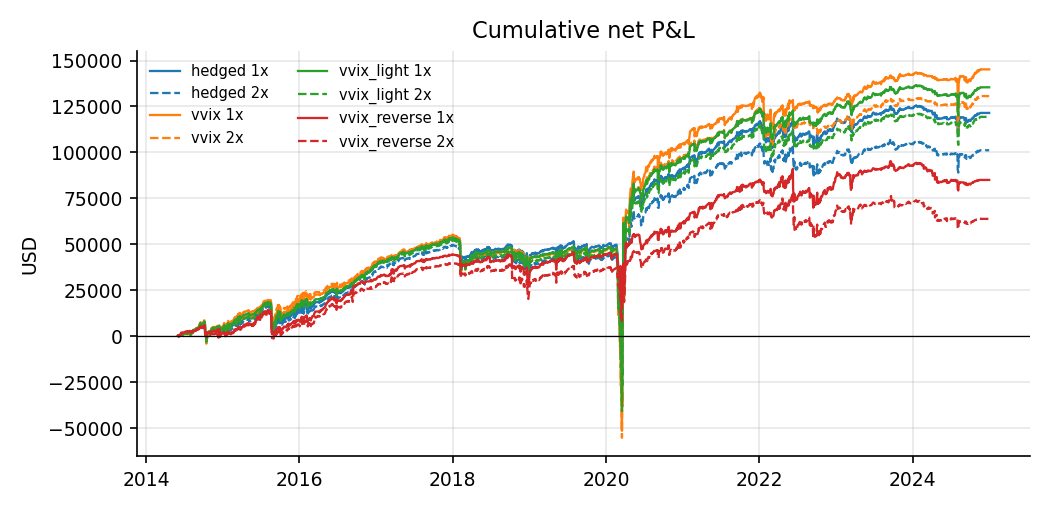
\includegraphics[width=0.92\linewidth]{figures/cum_pnl.png}\caption{Cumulative net P\&L, 1x solid and 2x dashed}\end{figure}

All four books track each other until February 2020. The up-tilted books fall further in the crash and recover further after it. From 2021 the lines move in parallel, with \texttt{vvix} keeping most of the lead it gained in 2020.

\begin{figure}[H]\centering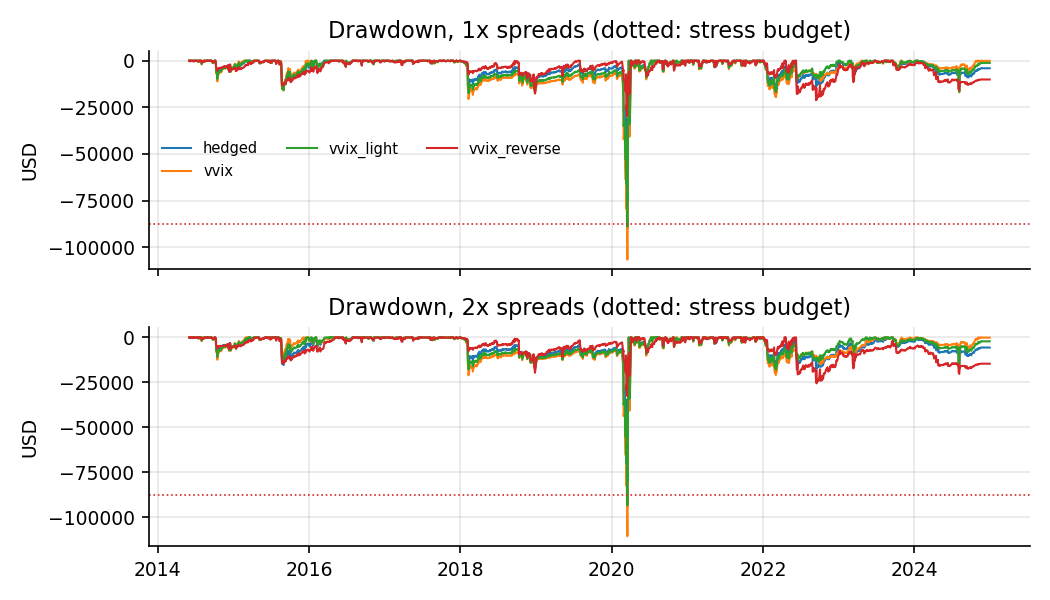
\includegraphics[width=0.92\linewidth]{figures/drawdown.png}\caption{Drawdown at 1x and 2x spreads; dotted line: the \$87,500 stress budget}\end{figure}

Every book has its maximum drawdown in the same episode: from the January 2018 equity peak to 17 March 2020. Only the 2020 trough crosses the budget line. Outside that episode, drawdowns are below about \$21k for all four books.

\begin{figure}[H]\centering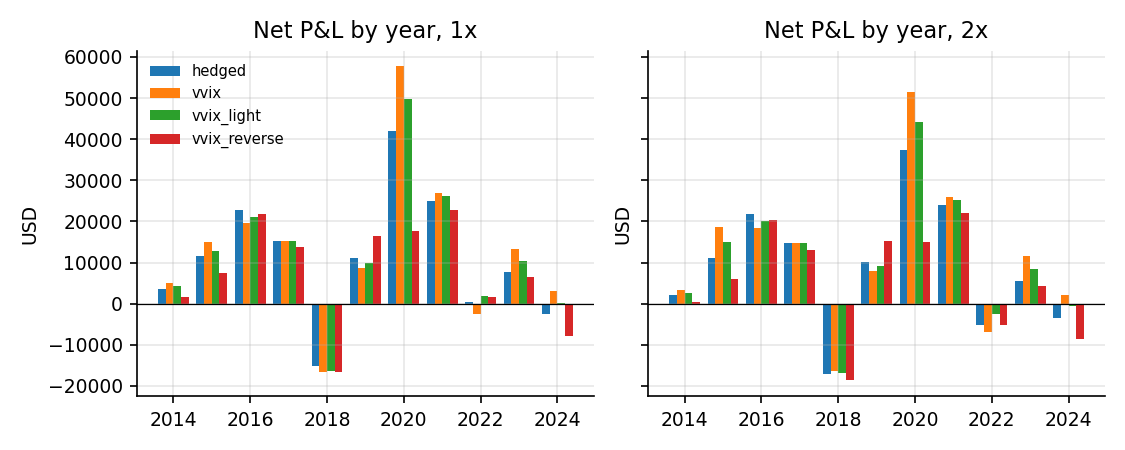
\includegraphics[width=0.92\linewidth]{figures/yearly.png}\caption{Net P\&L by year}\end{figure}

2020 explains most of the difference: \texttt{vvix} made \$15.7k more than \texttt{hedged} that year at 1x. The other ten years add up to \$8.0k: positive in 2014, 2015, 2021, 2023 and 2024, flat in 2017, and negative in 2016, 2018, 2019 and 2022.

\begin{figure}[H]\centering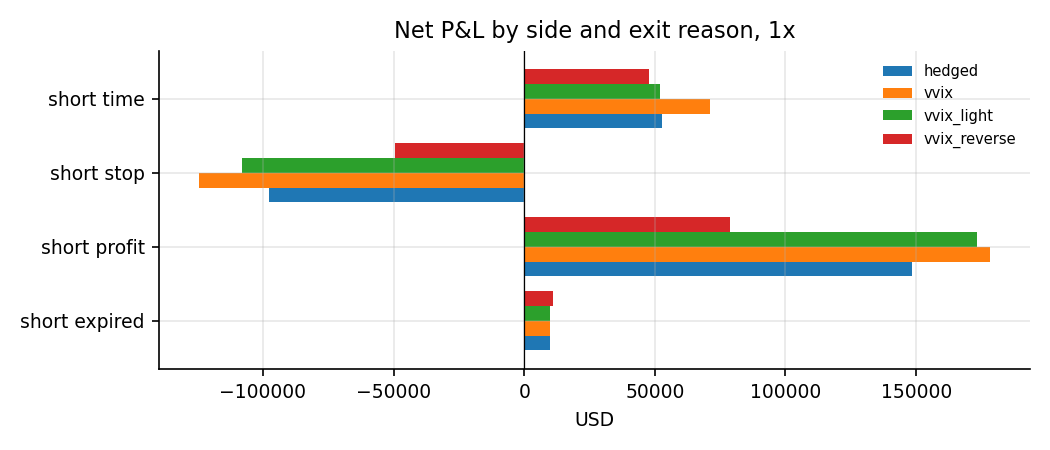
\includegraphics[width=0.92\linewidth]{figures/by_reason.png}\caption{Net P\&L by side and exit reason, 1x}\end{figure}

The up-tilt makes both stops and profit-takes bigger. Its stop losses are \$27k worse than \texttt{hedged}'s, its profit-takes \$30k better and its time exits \$18k better. The reverse tilt shrinks all three.

\begin{figure}[H]\centering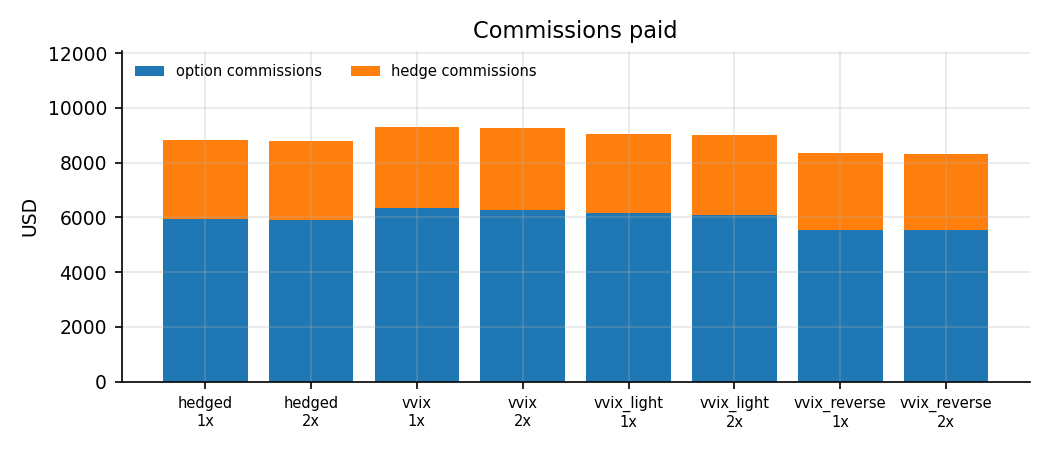
\includegraphics[width=0.92\linewidth]{figures/fees.png}\caption{Commissions paid}\end{figure}

Commissions scale with contracts and barely differ: \texttt{vvix} pays \$472 more than \texttt{hedged} over ten years at 1x.

\begin{figure}[H]\centering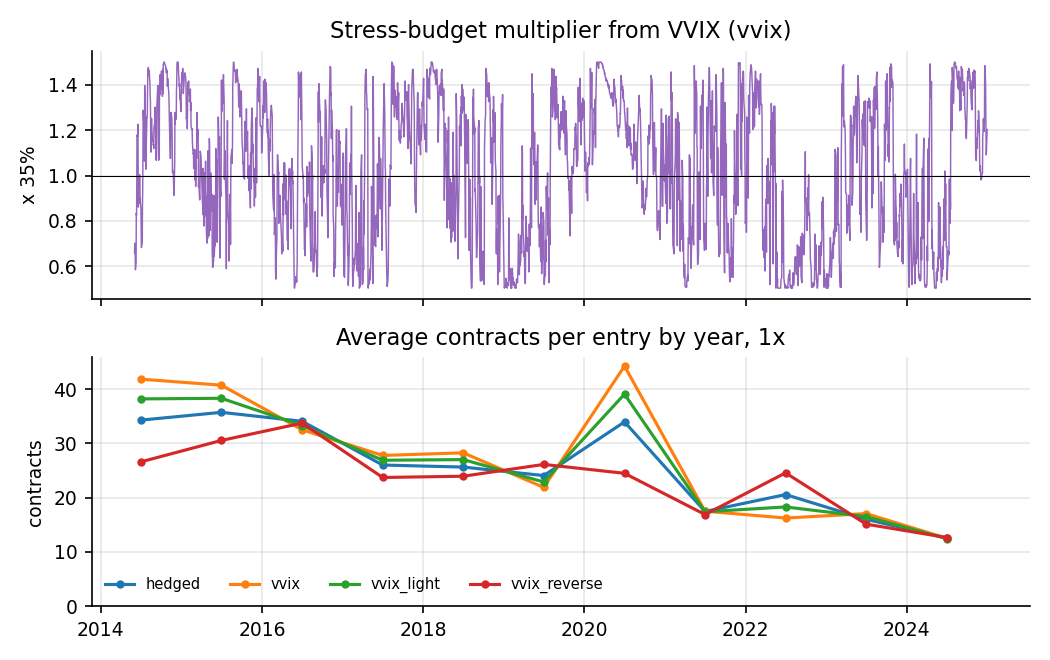
\includegraphics[width=0.92\linewidth]{figures/multiplier.png}\caption{Budget multiplier from VVIX (top) and average contracts per entry by year (bottom)}\end{figure}

The multiplier swings between 0.5x and 1.5x within months, so over a year it averages close to 1x. The mean at entry was 1.03x-1.04x in every book. Contracts differ most in 2014-2015 and 2020, the years VVIX sat high in its one-year range.

\section{Analysis}

\textbf{The tilt mostly acts as leverage on the March 2020 crash.} The book made five entries between 15 February and 30 April 2020, in every variant. All five came with VVIX near the top of its one-year range, so \texttt{vvix} opened them at 1.39x to 1.5x the fixed budget.

\begin{itemize}

\item The first two entries were stopped out in the selloff. The third, opened about ten days before the market low, made the largest gain of the decade in both books.

\item Over that window \texttt{vvix} made \$10.7k more than \texttt{hedged} at 1x. That is 45\% of its full-window lead (daily P\&L over the window; the five round trips' own net gives \$10.3k, 43\%).

\item The same larger size sent its drawdown to \$106.6k, against \$70.4k for \texttt{hedged}. The two books share the same peak (2 January 2018) and trough (17 March 2020).

\item This is mechanical. VVIX and IV were both at extremes, and the stress rule already sized up into high IV (2026-10-22). The tilt adds up to 50\% on top.

\end{itemize}

\textbf{Outside the crash, the tilt adds a little P\&L at slightly more risk.} With 15 February to 30 April 2020 left out (1x):

\begin{center}\small
\begin{tabularx}{\linewidth}{l l >{\raggedright\arraybackslash}X}
\toprule
\textbf{} & \textbf{\texttt{vvix}} & \textbf{\texttt{hedged}} \\
\midrule
Net P\&L, 1x & \$112.8k & \$99.9k \\
Max drawdown & \$20.5k & \$16.4k \\
ES & \ensuremath{-}\$2,338 & \ensuremath{-}\$2,224 \\
Sharpe & 0.83 & 0.81 \\
\bottomrule
\end{tabularx}
\end{center}

That is about \$13k over ten years. It is spread unevenly: \texttt{vvix} trailed \texttt{hedged} in four of the ten other years (2016, 2018, 2019, 2022), and 2023-2024 supplied \$11.2k of it. It is not enough to call the signal real.

\textbf{VVIX did not sort per-contract P\&L the way Park (2015) predicts.} In the reference book, the mean net P\&L per contract by VVIX tercile at entry was:

\begin{center}\small
\begin{tabularx}{\linewidth}{l >{\raggedright\arraybackslash}X}
\toprule
\textbf{VVIX tercile} & \textbf{Mean net P\&L per contract} \\
\midrule
Lowest & \$5.7 \\
Middle & \$25.7 \\
Highest & \ensuremath{-}\$0.1 \\
\bottomrule
\end{tabularx}
\end{center}

The top tercile still made \$55.8k in total because its largest trades won, including the 2020 crash trades, while its average trade was flat per contract. The reverse tilt fits the leverage reading. It cut P\&L by 30\%, the tail by 17\% and the drawdown by 58\%, and left Sharpe about where it was (0.55 against 0.52 at 1x, 0.40 against 0.43 at 2x).

\section{Verdict}

\textbf{Failed} on the pre-registered bar. P\&L rose, but the drawdown broke the stress budget at both spreads, the tail grew 19\%, and 2014-2019 at 1x was worse.

Don't promote and don't run the hold-out. The result says VVIX scaling is a way to take more crash risk, not a better signal for when puts pay. A follow-up would need its own card, for example a tilt capped at 1x (size down on calm VVIX only). Its gain would be small.

\section{Caveats}

\begin{itemize}

\item \textbf{In-sample:} the idea comes from the 2026-10-31 strategy research report (literature), and the book is the 2026-10-22 primary, chosen after its results. Before pre-registration, Claude saw the reference book's contracts per entry by year and the multiplier path, but not its P\&L by multiplier.

\item \textbf{One crash decides it:} half the lead comes from five entries in February to April 2020. A different path through that month (for example, a stop one day later) would change the result.

\item \textbf{Concentration overlaps with IV:} VVIX and IV were both high in the crash, so this test cannot separate a VVIX effect from the IV effect already in the stress rule.

\item \textbf{Spread model:} fitted on about two weeks of calm 2026 live quotes. Fills of up to 150 contracts in March 2020 use the same model as one contract. The 2x run is the stress test.

\item \textbf{Margin:} not modelled. The 2026-10-22 report estimated Reg-T margin above capital on 16 entries at the fixed budget; a 1.5x budget makes this worse.

\item \textbf{Data gaps:} about 3.3\% of scheduled times are skipped. \texttt{vvix\_\allowbreak{}reverse} had 14 unfilled orders at 1x against 9 in the other books, from path differences.

\end{itemize}

\section{Trials}

\textbf{This experiment:} 6 trials (3 variants \ensuremath{\times} 1x and 2x, one run of \texttt{experiment.\allowbreak{}py} at commit 954824c), plus the baseline's 2. The \texttt{hedged} reference was reused (2 trials, not rerun). The registry holds 98 trials after the four 2026-11-02 experiments.

\textbf{\texttt{-\allowbreak{}dirty} tags:} the two \texttt{vvix\_\allowbreak{}reverse} rows are tagged \texttt{954824c-\allowbreak{}dirty}. Three other experiments ran at the same time in the same working tree, and their new figure folders made the tree dirty. The engine, configs and this experiment's script were unchanged from 954824c during the run.

\textbf{Rebuild:} after the run, the yearly chart's legend was moved clear of the bars, and the figures were rebuilt with \texttt{-\allowbreak{}-\allowbreak{}report-\allowbreak{}only}, which adds no trials.

The pass bar was not changed.

\end{document}
